\section{Introduction} \label{sec:intro}
FPGAs have been increasingly utilized for accelerating data intensive applications 
such as neural network \cite{Zhao2017accelerating, Zhang2017improving,
Zhang2017frequency, guan2017fpdnn}, data compression \cite{fowers2015scalable} 
and graph processing \cite{Dai2017foregraph, zhou2016high} and gain increasing 
popularity over the years. This encourages more and more cloud vendors to integrate FPGAs 
in the cloud and provide FPGAs as a service \cite{f1, nimbix, baidu-cloud, aliyun, supervessel}. 
At the same time, high level design tools 
and integrated environments are increasingly provided to make the FPGAs accessible to 
high-level application designers and to improve the design productivity of 
the designers as well. However, optimizing the high level design for 
optimized performance remains challenging. To that end, we take 
BFS as an example exploring the high level data intensive application 
optimization on the FPGAs using state-of-art high level design tools. 
 
Breadth-first search (BFS) is the basic building component of graph processing and 
is thus of vital importance to high-performance graph processing. Nevertheless, 
it is notoriously difficult for accelerating on parallel 
computing architectures because of the irregular memory access and the low 
computation-to-memory ratio. At the same time, BFS on large graphs also involves 
tremendous parallelisms which indicates great potential for acceleration. 
With both the challenge and the parallelization potential, 
BFS has attracted a number of researchers exploring the acceleration on FPGAs 
\cite{attia2014cygraph, betkaoui2012reconfigurable, Dai2017foregraph, Ma2017fpga,
umuroglu2015hybrid, oguntebi2016graphops, engelhardt2016gravf, zhou2016high}. 

Previous work have shown that BFS accelerators on FPGAs can provide competitive  
performance and superior energy efficiency when given comparable memory bandwidth. 
However, these work typically optimize BFS or relatively general graph processing 
with dedicated circuit design using hardware description language (HDL). The HDL 
based designs with customized circuits are beneficial to the performance 
and save resource consumption, but it usually takes long time for development, 
upgrade, maintenance and porting to a different FPGA device with 
different resource constraints such as memory bandwidth, which are all 
important concerns from the perspective of the accelerator developers. Another 
engineering yet non-trivial problem is the high barrier to use the FPGA powered graph 
processing accelerators in high-level applications such as 
big data analytics, which is mostly caused by the lack of 
well-defined high level interface and user-friendly SDK supporting 
various hardware systems. While improving the ease of using the 
HDL based accelerators requires a lot of design efforts, we believe 
that this is actually one of the key obstacles hindering the 
widespread adoption of the FPGA accelerators despite the great 
performance-energy efficiency advantages.

To alleviate this problem, more and more people from both industry and 
academia opt to use high level synthesis (HLS) design tools for 
developing accelerators of their target applications namely 
accelerating with software programmable FPGAs \cite{koch2016fpgas}. 
We argue that using HLS for hardware design is not only improving 
the productivity of the designers, it is also 
beneficial to the high-level application users when the HLS based 
FPGA designs get continuous and steady FPGA and cloud vendor support.

Under such a context, we focus on BFS accelerator design and 
optimization using SDAccel which is a standard high level design tool targeting 
the data-center application acceleration leveraging FPGAs provided by Xilinx. 
As BFS is known to be memory bandwidth bound, we thus centers the memory 
access optimization while exploring the FPGAs for BFS acceleration. With intensive 
experiments on memory access patterns of BFS on large graphs, we observe 
that there are both considerable random memory access, short sequential read 
and long sequential read in different parts of the BFS algorithm. 
For long sequential read, we use the stream model to ensure the design 
tools to produce efficient burst memory access. At the same time, we also
explore the data width optimization and data path duplication 
for higher memory bandwidth utilization. For the time-consuming 
short sequential and random memory access, we squeeze the 
unnecessary memory access by removing the redundant memory operations first. 
Then we take advantage of the data locality and develop a specific cache for 
efficient random vertex status access. 

According to the experiments on a set of big graphs, the optimized high level BFS 
accelerator obtains up to 60X performance speedup when compared to the baseline 
design. Although there is still a moderate performance gap compared to previous 
optimized HDL based design, the HLS based design has better software-like features 
in terms of portability, ease of use and maintenance.

The major contributions of this work are summarized as follows.
\begin{itemize}
    \item As far as we know, this is the first HLS based BFS accelerator on 
        FPGAs targeting portability and ease of use on top of performance. 
    \item With intensive experiments, we explored the memory access 
        patterns of the BFS accelerator and exhibited the potential 
        optimization opportunities.
    \item With the observations of the memory access characteristics of BFS, we 
        developed a series of BFS accelerator optimization strategies such 
        as pipeling, caching and prefetching using a standard HLS tool.
        The resulting accelerator shows significant performance speed up 
        over a baseline HLS design.
\end{itemize}

This rest of the paper is organized as follows. In Section \ref{sec:relatedwork}, 
we brief the background of software programmable FPGAs and related work of 
BFS acceleration especially on FPGAs. In Section \ref{sec:observation},  
we analyze the BFS memory access pattern and motivate the BFS accelerator 
optimizations in this work. In Section \ref{sec:overview}, we present 
the overview of the BFS accelerator design using the SDAccel design environment. 
In Section \ref{sec:bfs-opt}, we detail the proposed high level BFS accelerator 
design and optimizations such as pipiling and caching. 
In Section \ref{sec:experiment}, we present comprehensive experiments of the 
BFS accelerator. Finally, we conclude this work in Section \ref{sec:conclusion}.

\section{Background and related work} \label{sec:relatedwork}
In this section, we briefly introduce the evolving FPGA 
cloud and software programmable FPGAs.
Then we review the existing BFS acceleration work and introduce the widely 
used BFS algorithm for the BFS accelerator design.

\subsection{FPGA Cloud and software programmable FPGAs}
With the increasing demand of FPGAs on many data intensive 
applications such as software defined network 
\cite{zhang2017scalable, li2016clicknp}, neural 
network \cite{Zhao2017accelerating, Zhang2017improving}, 
and database \cite{wang2017relational}, more and more 
cloud vendors start to provide FPGA as a service. However,
HDL based FPGA design method suffers low design productivity, 
expensive reuse, portability and maintenance cost as well 
as ease of use problem. Programming FPGAs remains a critical 
obstacle hindering the adoption of FPGAs in more domains 
of applications. 

To address this problem, the cloud vendors and FPGA vendors have started 
to offer high level programming options such as C/C++ and OpenCL. The high 
level design tools and environments make it possible to program FPGAs 
without much low-level hardware design experiences \cite{nimbix, xilinx-sdaccel, intel-opencl}. 
In particular, these software programmable FPGAs are moving forward to the FPGA cloud
rapidly. Xilinx Nimbix \cite{nimbix} already have OpenCL and high level 
synthesis (HLS) tools supported. Amazon is also moving forward to this 
direction \cite{f1}. Despite the performance penalty and higher resource consumption, 
it can be forseen that the evolving HLS tools \cite{Nane2016hls-survey} making 
FPGAs accessible to more software designers will become increasingly important 
in future.

In line with this trend, we use SDAccel \cite{xilinx-sdaccel} to develop the 
BFS accelerator for the sake of better portability and higher design 
productivity. Figure \ref{fig:sdaccel} presents the SDAccel overview. 
It is a design environment targeting x86-Based server + PCIe 
based FPGA acceleration card. With the integrated libraries, 
it handles both the drivers and run-time environment such that 
the designers can focus on the computing kernel design on FPGA with either 
C/C++ based HLS or OpenCL. In addition, the same design can be seamlessly 
ported to other FPGAs with SDAccel support such as the FPGAs in 
Xilinx Nimbix Cloud \cite{nimbix}.

\begin{figure}
\center{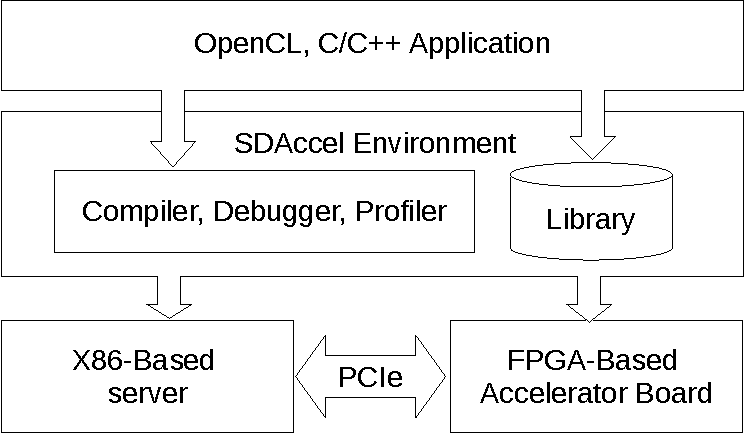
\includegraphics[width=0.75\linewidth]{sdaccel}}
    \caption{Xilinx SDAccel design framework \cite{xilinx-sdaccel}}
\label{fig:sdaccel}
\end{figure}


\subsection{BFS Algorithm}
BFS is a widely used graph traversal algorithm and it is the basic 
building component of many other graph processing algorithms. 
It traverses the graph by processing all vertices with the same distance from the 
source vertex iteratively. The set of vertices which have the same distance from the 
source is defined as frontier. The frontier that is under analysis in the BFS iteration 
is named as current frontier while the frontier that is inspected from current frontier 
is called next frontier. By inspecting only the frontier, BFS can be implemented efficiently 
and thus the frontier concept is utilized in many BFS implementations.

BFS algorithm can be formalized as follows. Assume $G$ is a graph with vertex 
set $V$ and edge set $E$, BFS finds a shortest path from a source vertex
$v_s \in V$ to all the other vertices in the graph $G$. For each vertex $v \in V$, 
BFS will output a level value $l$, indicating its distance from $v_s$ ($v$ can be accessed 
from $v_s$ by traveling through $l - 1$ edges. 

A widely used frontier based BFS algorithm implementation is named as 
level synchronous BFS \cite{attia2014cygraph, betkaoui2012reconfigurable, 
zhang2017boosting}. The details of the algorithm are presented in 
Algorithm \ref{alg:level-bfs}.
The basic idea is to traverse the frontier vertices and inspect the neighbors 
of the current frontier vertices to obtain the frontiers in next BFS iteration. 
Then the algorithm can start a new iteration with a simple switch of 
current frontier queue and next frontier queue. The algorithm ends when 
the frontier queue is empty.

\begin{algorithm}
    \small
	\caption{Level Synchronous BFS Algorithm} \label{alg:level-bfs}
	\begin{algorithmic}[1]
		\Procedure{BFS}{}
		\State $level[v_k] \gets -1$ where $v_k \in V$
		\State $level[v_s] \gets 1$
		\State $current\_frontier \gets v_s$
		\State $current\_level \gets 1$
		\While {$current\_frontier$ not empty} 
		\For{$v \in current\_frontier$}
		\State $S \gets {n \in V | (v, n) \in E}$
		\For {$n \in S$}
		\If {$level[n] == -1$}
		\State $level[n] \gets current\_level + 1$
		\State $next\_frontier \gets n$
		\EndIf
		\EndFor
		\EndFor
		\State $current\_level \gets current\_level + 1$
		\State Swap $current\_frontier$ with $next\_frontier$
		\EndWhile
		\EndProcedure
	\end{algorithmic}
\end{algorithm}

\subsection{Related work}
The growing importance of efficient BFS traverse on large graphs 
have attracted attentions of many researchers. In the past few years, 
many BFS optimization algorithms and accelerators have been proposed 
on almost all the major computing platforms including multi-core processors, 
distributed systems, GPUs and FPGAs. In this work, we will 
particularly focus on the FPGA based BFS acceleration. 

The researchers tried to explore BFS acceleration 
on FPGAs from many various angles.
To alleviate the memory bandwidth bottleneck of the 
BFS accelerators, the authors in \cite{zhang2017boosting} 
explored the emerging Hybrid Memory Cube (HMC) which provides 
much higher memory bandwidth as well flexibility for BFS 
acceleration, while the authors in \cite{attia2014cygraph} 
proposed to change the compressed sparse row (CSR) format slightly. 
Different from the first two work, the authors in \cite{umuroglu2015hybrid} 
choosed to perform some redundant but sequential memory access for higher memory bandwidth 
utilization based on a spare matrix-vector multiplication model.
In addition, they particularly took advantage of the 
hybrid CPU-FPGA architecture offloading only highly parallel 
BFS iterations for FPGA acceleration while leaving the rest 
on host CPU.  

Most of the BFS accelerators are built on a vertex-centric 
processing model, while the authors 
in \cite{zhou2016high} explored the edge-centric graph processing and demonstrated 
significant throughput improvement. On top of the single FPGA board acceleration, 
the authors in \cite{attia2014cygraph, betkaoui2012reconfigurable} also explored 
BFS acceleration on a FPGA based high performance computing system with multiple 
FPGAs and memory instances. There are also work exploring customized soft processors 
for graph processing and building a distributed solution on 
top of a group of embedded FPGA boards \cite{kapre2015custom, wang2010message}.

Instead of building specialized BFS accelerator, many researchers opted to develop 
more general graph processing accelerator framework or library 
recently \cite{engelhardt2016gravf, oguntebi2016graphops, Dai2017foregraph, dai2016fpgp}. 
They can also be utilized for BFS acceleration despite the lack of 
specialized optimization for BFS. Meanwhile, this is also a way to improve 
the ease of use FPGAs for graph processing acceleration.

Prior BFS acceleration work have demonstrated the potential benefits of accelerating 
BFS on FPGAs. These accelerators were mainly developed for the sake 
of performance and generality for more graph processing algorithms. 
However, they were all hand-crafted HDL designs and applying these accelerators 
on high level applications for software designers still requires a lot of 
efforts especially when the target computing platforms are different. 
To that end, we opt to develop HLS based BFS accelerators 
using SDAccel such that the accelerator packed in an 
OpenCL thread can be easily utilized in high level applications 
by a \textit{software designer}. Meanwhile, the same design can be easily 
ported to other FPGAs with the SDAccel support with negligible 
engineering efforts.

\section{Observations on BFS memory access} \label{sec:observation}
BFS on large graphs is known to be a memory bandwidth bound task. 
Therefore understanding the BFS memory access pattern and providing suitable memory 
access optimization strategies is critical to make best use of the memory bandwidth 
and achieve higher performance. Therefore, we analyzed the memory access 
pattern of the level synchronous BFS on a Youtube graph \cite{yang2012defining}.
The observations can be used to guide the BFS optimization in this work.

\textit{Observation 1: BFS memory access pattern is rather complex. 
It involves considerable short sequential memory accesses 
and random memory accesses which are usually quite 
expensive. At the same time, it also includes quite some long 
sequential memory accesses and the overall access time can't be 
ignored due to the relatively large memory access amount.} We analyzed the 
memory access pattern of the BFS on Youtube Graph. The burst length distribution 
of the memory accesses is presented in Figure \ref{fig:burst-len-youtube}. 
(In FPGA design, longer sequential memory access can be usually taken as burst 
transfer from the perspective of an internal bus. We use 
the burst and sequential access interchangeably in this paper.)
It can be found that there are a large amount of random and short sequential 
memory access. Meanwhile, we notice that shorter burst length especially 
the random memory access results in extremely low memory bandwidth 
when compared to that of longer sequential memory access. Worse still, 
more parallel data paths with the typical data width i.e. 32-bit will 
not improve the memory bandwidth utilization too much due to the memory 
access conflict, which makes the random and short sequential 
memory access optimization difficult. Note that the memory bandwidth is obtained 
from a separate HLS based memory test on an Alpha Data ADM-PCIE-7v3 FPGA card.
We use the test result to estimate the memory access time of BFS. 
In general, it can be concluded that the short sequential and random 
memory access are the most critical part of the BFS memory accesses. 
 
\begin{figure}
\center{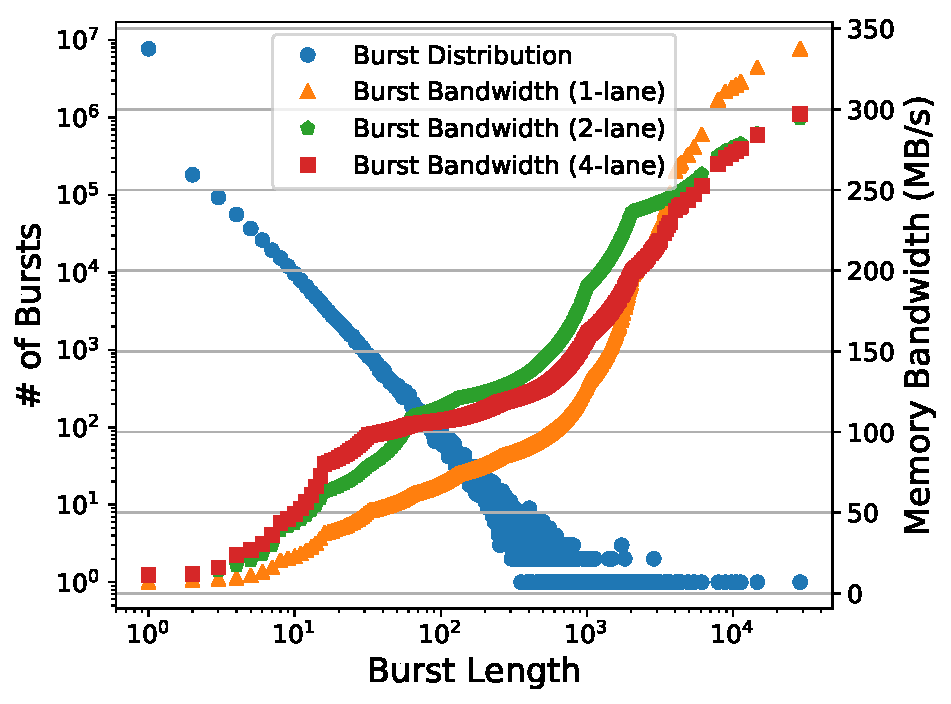
\includegraphics[width=0.85\linewidth]{burst_len_youtube}}
\caption{Burst length distribution in BFS on Youtube Social Network Graph. 
    Random memory access and short sequential memory access take up the 
    the majority of the memory access overhead of BFS. Multiple parallel 
    lanes of data paths improve the memory bandwidth utilization when the 
    burst lenght is relatively large, but they will not help much 
    for short or random memory accesses.}
\label{fig:burst-len-youtube}
\end{figure}

\textit{Observation 2: There are many redundant vertices in the 
frontier vertex neighbors leading to a lot of redundant memory access in BFS.} 
As random memory access takes up a big portion of the overall memory 
access overhead, we further investigate the random memory access in BFS. 
According to the level synchronous BFS algorithm, the random memory access mainly comes 
from the frontier neighbor vertex status read/write. 
However, many frontier vertices may have common neighbor vertices and these common 
vertices lead to many redundant vertex status read. To gain insight of the neighbor 
vertex redundancy of different frontier vertices, we compare the total amount of frontier 
neighbor vertices and the amount of unique frontier neighbor vertices in each BFS iteration.
(Note that we use the Youtube graph as an example in the experiment as well.) 
The comparison is shown in Figure \ref{fig:repeat-neighbor} and it can be clear that 
the BFS iterations with the largest amount of frontier neighbors include a lot of redundant 
vertices. The redundancy proportion even goes up to 80\% in the largest BFS iteration. 
With proper redundancy removal strategy,
the vertex status reads in the following part of the BFS can be reduced dramatically.

On top of the redundant vertices, the visited vertices in previous 
BFS iterations don't need to be checked by reading the vertex status 
from memory. According to our experiment, the visited frontiers 
take up quite some of the total frontier neighbor vertices. However, this is 
observed in only one of the BFS iterations. It indicates that buffering 
frontier vertices may help to avoid unnecessary random vertex status read, 
but the benefit can be marginal.    

\begin{figure}
\center{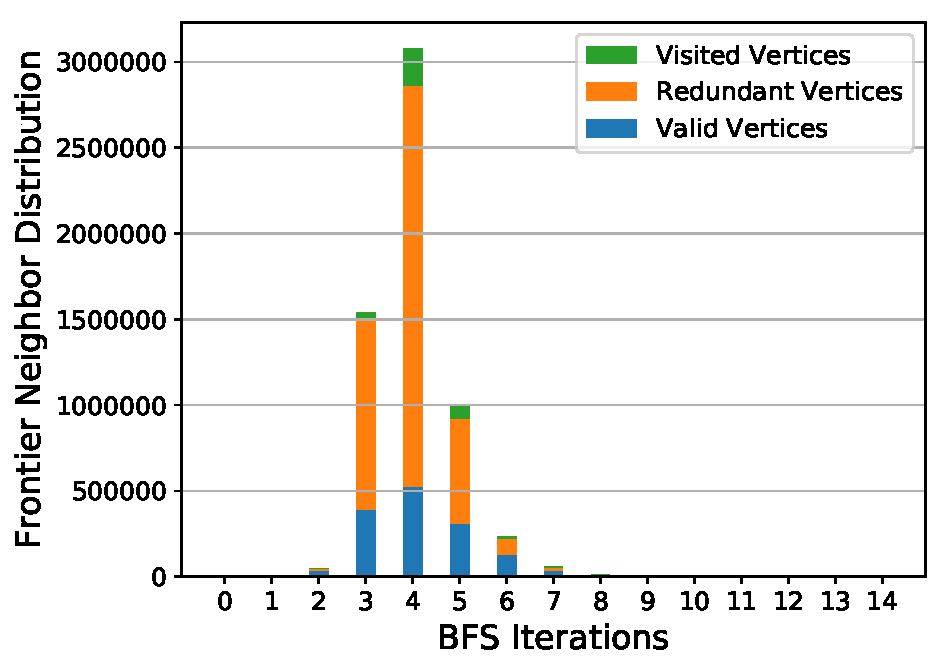
\includegraphics[width=0.85\linewidth]{neighbor_vertex}}
\caption{Unnecessary random vertex status read decomposition. 
    Majority of the frontier neighbor vertices are 
    redundant and another portion of vertices are already 
    visited in previous BFS iterations.}
\label{fig:repeat-neighbor}
\end{figure}

\textit{Observation 3: The vertex status reads have good 
spatial locality especially when the redundant access are removed in advance, 
but the temporal locality is relative bad meaning that the status reuse 
distance is quite long.}
Another potential optimization of random memory access is to use cache architecture, 
which explores the data locality and improves memory bandwidth utilization 
accordingly. To ascertain the feasibility of using cache, we analyzed both the 
temporal and spatial locality of the vertex status reads. Since 
the frontier neighbor vertex redundancy removal affects the locality, 
we also did the spatial locality analysis on a redundancy-free 
vertex status read sequence. The data locality based cumulative 
distribution function (CDF) curve is shown in 
Figure \ref{fig:youtube-locality}. We can find that there are actually 
very good spatial locality in general. In particular, the spatial 
locality gets even better and over 70\% of the vertices have reference distance 
less than 200 when the redundancy is squeezed. The temporal locality is not as 
good and only around 20\% of the accesses have short reuse distance. In general, 
we still believe that a specialized cache is beneficial to the random 
vertex status reads. Note that we use 
the stride distance as the metric of spatial locality and reuse distance as the metric 
of temporal locality \cite{weinberg2008chameleon}. The stride distance of a reference 
to address A is defined as the minimum distance between A and the 
memory addresses in a lookback window right before the current 
memory access. We set the loopback window to be 32 in the experiment. 
The reuse distance of some reference to 
address A is equal the number of unique memory addresses that have been 
accessed since the last access to A.  

\begin{figure}
\center{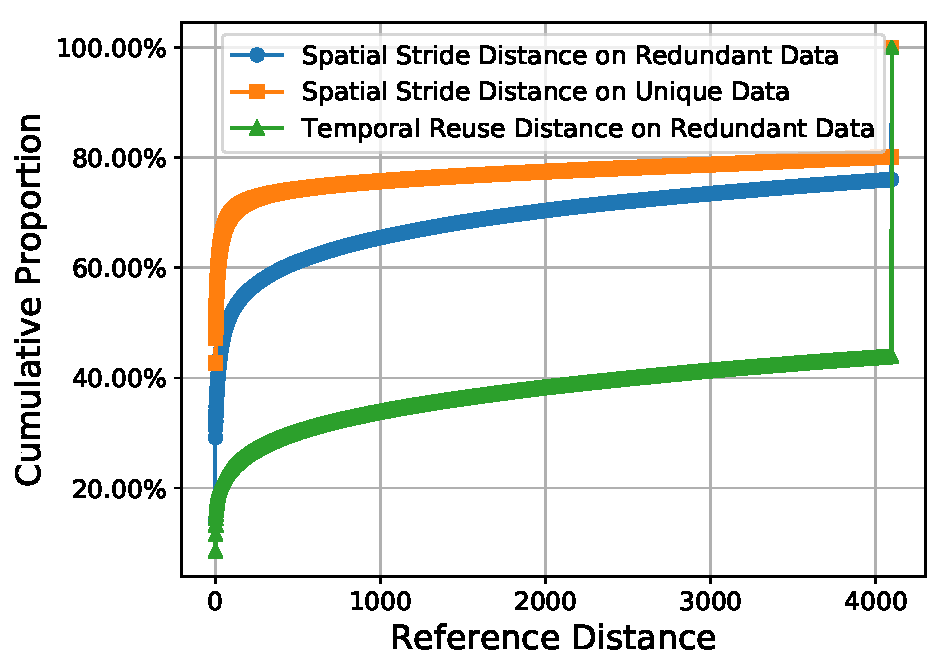
\includegraphics[width=0.8\linewidth]{youtube-locality}}
\caption{Cumulative Distribution Function (CDF) of reuse distance 
    and stride distance. They stand for the temporal locality and spatial 
    locality of the BFS vertex status reads respectively. Note that the 
    reference distance larger than 4000 is combined as they are difficult 
    to be optimized in hardware design.}
\label{fig:youtube-locality}
\end{figure}

%\textit{Observation 4: In the skewed graphs, a small amount of high degree vertices 
%covers a big proportion of the connections (edges) in the graph.}
%The real-world graphs usually have large amount of vertices and adges while 
%the FPGA on chip memory is far from enough for caching and buffering. 
%Hereby, only a sub set of them can reside in on-chip memory at runtime. 
%It can be expected that high degree vertex related information 
%are more likely to be referenced in 
%the BFS iterations. To further investigate the potential of buffering 
%the high degree vertices, we analyzed the vertex degree distribution 
%of Youtube graph. The vertex degree based CDF and vertex based 
%CDF is shown in Figure \ref{fig:degree-distribution}. The two CDF curves in the figure 
%exhibit that the top 10\% high degree vertices include more than 70\% of 
%vertex degree namely edges in the graph. Basically keeping these high degree 
%vertex infomration such as vertex status on chip can avoid the repeated 
%vertex staus checking in BFS and is benefitial to the memory access efficiency. 
%Another thing that is worth for highlighting is the one degree vertex distribution.
%It takes up over 40\% of the overall amount of the vertices in the graph. In BFS, 
%the status of these vertices will be read and write only once.  
%
%\begin{figure}
%\center{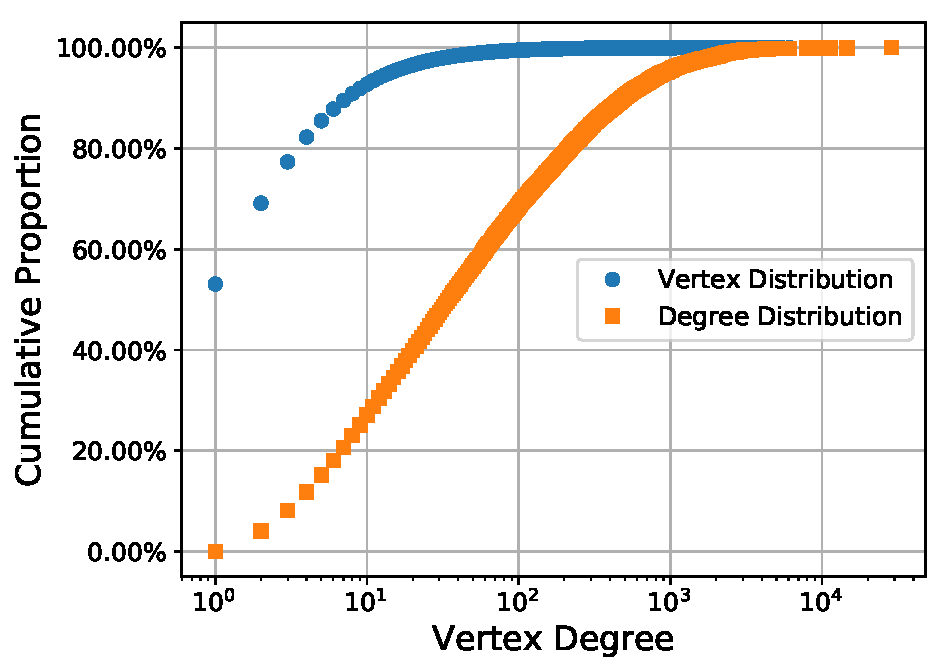
\includegraphics[width=0.9\linewidth]{degree-dist}}
%\caption{Vertex Degree Distribution. A small amount of 
%    high degree vertices take up a large portion of the connections in the graph.}
%\label{fig:degree-distribution}
%\end{figure}

In summary, we notice that random and short sequential memory accesses 
are the most time-consuming part of the overall BFS memory accesses. 
Although it is generally difficult to optimize these memory accesses, 
we observe that large amount of redundancy exists and 
the data exhibit very good spatial locality. Taking advantage of the 
memory access characteristics, we may optimize the BFS memory accesses 
greatly and improve the BFS performance eventually.

\section{BFS Accelerator Overview} \label{sec:overview}
Our BFS accelerator follows a vertex based processing paradigm 
and the bulk synchronous parallel (BSP) model utilized in many previous 
graph processing frameworks \cite{malewicz2010pregel}. In particular, 
it targets in-memory graphs on a PCIe based high performance FPGA card. 
Basically, it has the whole graph stored in FPGA DDR with a standard 
CSR format and does the BFS on FPGA without any interference from the host CPU. 

The BFS algorithm is critical to the BFS accelerator and we explored the 
existing level synchronous BFS algorithm in detail. We notice that 
the level synchronous BFS algorithm may have redundant vertices pushed to the 
frontier queue in a parallel architecture especially when the frontier grows larger.
The main reason roots in the large amount of overlapped neighbor vertices among the 
frontier vertices as mentioned in previous section. When the frontier neighbors 
are inspected in parallel for faster BFS traverse, these overlapped vertices may be 
considered as frontiers independently and inserted into the next frontier queue. 
As a result, there may be redundant vertices put into the frontier queue and it is 
rather complex to get rid of the redundancy \textit{completely}. Although the redundant 
vertices in the frontier will not cause any BFS mistakes, they will soon lead to large 
amount of redundant traverses recursively and degrade the BFS performance.

To address this problem, we analyze the frontier from the 
vertex status in each BFS iteration to completely cut down the 
propagation of the redundant frontier vertices as proposed in prior 
GPU based BFS acceleration \cite{liu2015enterprise}. The modified algorithm is described 
in Algorithm \ref{alg:modified-bfs}. Instead of inspecting on the frontier vertices directly, 
it starts with vertex status analysis and inspects the frontier 
in each BFS iteration. Although it seems the additional frontier inspection stage 
brings more memory access, the inspection processing are complete sequential 
memory access and can be done efficiently. It is still worth for the overhead 
when compared to the cost caused by the redundant frontier vertices. 

\begin{algorithm}
	\caption{Modified BFS Algorithm} \label{alg:modified-bfs}
    \small
	\begin{algorithmic}[1]
		\Procedure{BFS}{}
		\State $level[v_k] \gets -1$ where $v_k \in V$
		\State $level[v_s] \gets 0$
		\State $current\_level \gets 0$
		\State $frontier \gets v_s$

        \While {$!frontier.empty()$} 

		\For{$v \in V$}
		\If{$level[v] == current\_level$}
		\State $frontier \gets v$
		\EndIf
		\EndFor

		\For{$v \in frontier$}
		\State $S \gets {n \in V | (v, n) \in E}$
		\For {$n \in S$}
		\If {$level[n] == -1$}
		\State $level[n] \gets current\_level + 1$
		\EndIf
		\EndFor
		\EndFor
		\State $current\_level \gets current\_level + 1$
		\EndWhile
		\EndProcedure
	\end{algorithmic}
\end{algorithm}

\section{HLS based BFS optimization} \label{sec:bfs-opt}
With the observations in Section \ref{sec:observation} 
and the modified BFS algorithm in Section \ref{sec:overview}, 
we start to optimize the BFS accelerator using high level design tools 
from a series of different angles including pipelining, redundancy 
removal, caching and prefetching. The optimizations are discussed in 
detail in the following sub sections.

\subsection{BFS pipelining}
The baseline BFS algorithm is a multi-level nested loop with 
dynamic memory accesses. It is quite challenging for the HLS 
tools to produce optimized hardware. In particularly, some of the 
long sequential memory access in BFS outer loops 
may fail to be inferred as burst memory operations by the HLS tools 
leading severe performance drop.
To address this problem, we divide the BFS algorithm into pipelined 
sub functions. The sub functions with sequential memory accesses 
can be explicitly optimized with PIPELINE pragma and we can ensure 
these sequential memory accesses to be synthesized as efficient 
burst memory operations. Meanwhile, the pipelined sub functions 
fit well with the data flow model of Vivado HLS, 
which explores the function level parallelism allowing the 
sub functions to overlap their operations.

The pipelined BFS algorithm is detailed in Algorithm \ref{alg:bfs-stream}. 
It consists of six sub functions 
labeled as f1 to f6. In f1, vertex status is read from 
FPGA DDR memory sequentially through a streaming port. 
When the vertex status is fetched, f2 inspects the status 
flowed from the stream buffer, decides the current frontier 
and dumps the frontier to the downstream pipeline. 
With the frontier stream, f3 can further fetch graph 
data stored as CSR. CSR includes a row pointer array (RPA) 
and a column index array (CIA), and they must be sequentially accessed. 
In f3, we combine each pair of RPA entry of the frontier as a construct 
and pass it to the next stream function f4. When f4 gets the RPA pair, 
it can read the CIA sequentially through a streaming port. 
When data in CIA stream which is essentially the potential 
next frontier vertices are received in f5, their vertex status 
will be checked by reading the vertex status array stored in DDR as well.
Only the vertices that are not visited yet will be further forwarded to the f6. 
In f6, the vertex status will be updated.

\begin{algorithm}
	\caption{Streamed BFS Algorithm} \label{alg:bfs-stream}
    \small
	\begin{algorithmic}[1]
        \Procedure {BFS}{}
        \State $frontier\_size \gets 1$
        \State $level \gets 0$
        \While {$(frontier\_size > 0)$}
        \State $f1(depth, depth\_stream)$
        \State $f2(depth\_stream, frontier\_stream, level, frontier\_size)$ 
        \State $f3(frontier\_stream, CSR.RPA, RPA\_stream)$
        \State $f4(RPA\_stream, CSR.CIA, CIA\_stream)$ 
        \State $f5(CIA\_stream, depth, next\_frontier\_stream)$
        \State $f6(depth, next\_frontier\_stream, level)$
        \State $level \gets level + 1$
        \EndWhile
        \EndProcedure
        \State

        \Procedure{f1}{$depth$, $depth\_stream$}
        \For {$v \in V$}
        \State $depth\_stream << depth[v]$
        \EndFor
        \EndProcedure

        \Procedure{f2}{$depth\_stream, frontier\_stream, level, frontier\_size$}
        \State $frontier\_size = 0$
        \For {$v \in V$}
        \State $d[v] \gets depth\_stream.read()$
        \If {$(d[v] == level)$}
        \State $frontier\_stream << v$
        \State $frontier\_size++$
        \EndIf
        \EndFor
        \EndProcedure

        \Procedure{f3}{$frontier\_stream, CSR.RPA, RPA\_stream$}
        \While {$(!frontier\_stream.empty())$}
        \State $v \gets frontier\_stream.read()$
        \State $RPA\_stream << [CSR.RPA[v], CSR.RPA[v+1]]$
        \EndWhile
        \EndProcedure

        \Procedure{f4}{$RPA\_stream, CSR.CIA, CIA\_stream$}
        \While {$(!RPA\_stream.empty())$}
        \State $[begin, end] \gets RPA\_stream.read()$
        \For {${v \in CSR.CIA(begin, end)}$}
        \State $CIA\_stream << v$
        \EndFor
        \EndWhile
        \EndProcedure

        \Procedure{f5}{$CIA\_stream, depth, next\_frontier\_stream$}
        \While {$(!CIA\_stream.empty())$}
        \State $v \gets CIA\_stream.read()$
        \If {$(depth[v] == -1)$}
        \State $next\_frontier\_stream << v$
        \EndIf
        \EndWhile
        \EndProcedure

        \Procedure{f6}{$depth, next\_frontier\_stream, level$}
        \While {$(!next\_frontier\_stream.empty())$}
        \State $v \gets next\_frontier\_stream.read()$
        \State $depth[v] \gets level + 1$
        \EndWhile
        \EndProcedure

    \end{algorithmic}
\end{algorithm}

According to the description of the streamed BFS algorithm, we notice that 
five sub functions involve external memory access and they have quite different 
memory access patterns. The memory access patterns are summarized in 
Figure \ref{fig:bfs-stream}. f3 reads all the vertex status and 
it has a long sequential memory read. f2 reads the CSR row pointer of the frontier, 
and it reads two sequential words each time. f1 reads the CSR column index and the 
burst length depends on the vertex degree which varies in a large range. 
f4 and f5 involves vertex status reads and writes of the next frontier vertices.
As these vertices are not sequential, the HLS tools just take them as random access 
without any specific hints from the designers. 

\begin{figure}
\center{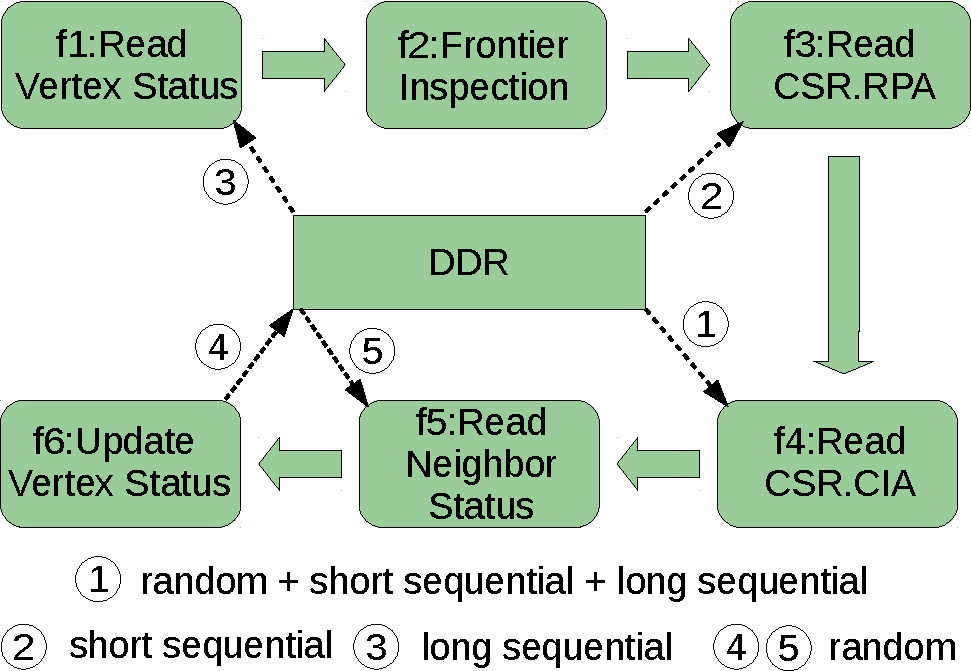
\includegraphics[width=0.65\linewidth]{bfs-stream}}
\caption{Streamed BFS Algorithm}
\label{fig:bfs-stream}
\end{figure}

\subsection{Memory Access Optimization}
As observed in Section \ref{sec:observation}, memory access espeically the random and 
short sequential memory accesses are critical to the 
BFS performance. In this sub section, we will mainly explore the memory 
access optimization techniques on top of the pipelined design.

\subsubsection{Redundancy Removal}
There are many redundant vertices among the frontier neighbors in BFS. 
They may further cause unnecessary vertex status reads and writes in 
f5 and f6 respectively. In order to remove the redundant memory access 
and improve the memory bandwidth utilization, we create hash tables 
to perform the redundancy removal. As the redundant vertices are 
relatively random, a big hash table can be utilized to squeeze 
the redundancy. However, big hash table degrade the hardware implementation 
frequency and eventually lower the overall performance. To address this problem, we 
build a series of smaller hash tables and apply them in parallel. 
The hash table based redundancy removal structure is shown in Figure \ref{fig:hash-strategy}. 
We use the lower bits of the data address as the hash function 
for the sake of better timing. An input data that fails to find a 
record in any of the hash tables will be considered to be a unique 
data and put into one of the hash tables to avoid repeated data 
going through the filter. In order to ensure balanced hash 
table utilization, we implement a hardware-friendly round robin 
arbiter to decide the hash table updating order. 
  
\begin{figure}
\center{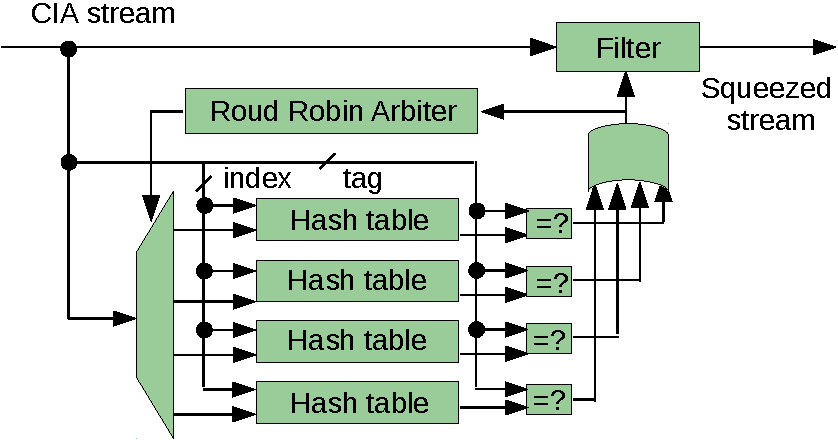
\includegraphics[width=0.75\linewidth]{hash-strategy}}
    \caption{Redundancy removal based on parallel hash tables.}
\label{fig:hash-strategy}
\end{figure}

\subsubsection{Cache Optimization}
According to the experiments in Section \ref{sec:observation}, 
there are many random memory access and short 
sequential memory access in f5 and f6. 
It is generally difficult to optimize these memory accesses. Fortunately, 
the spatial locality analysis shown in the observation experiments 
implies the great potential of cache based memory access optimization. 
Inspired by the observation, we developed an HLS based cache specifically 
for the vertex status \textit{depth} access. 

Since the cache is only used for \textit{depth} array read and write, we  
choose the \textit{depth} array index instead of its physical address for cache 
indexing. Each cache line is set to be 512-bit which is equal to the recommended 
memory access data width and a single memory read or write operation can 
fulfill the requirement of the cache operations including cache read miss, 
cache write miss and cache write back. Since the cache can't be shared 
between different SDAccel data flow functions, a natural cache design is 
to implement both cache in f5 and f6. Both cache can be relatively simple 
for supporting only read memory operations in f5 and writing memory operations in f6.  
 
\subsubsection{Prefetch optimization}
According to the BFS algorithm, the frontier is sequentially inspected. 
Therefore, the CSR information is also accessed in one direction 
in f3 and f4, though they are not necessarily sequential. Basically 
both the column array index and the row column index will increase 
monotonically in one BFS iteration. The spatial locality is 
good but there is no temporal locality. To optimize these memory 
accesses, a small prefetch cache 
is build to improve the memory access efficiency. 

Prefetch length setup is critical to the performance of the resulting design.
A longer prefetch improves the hit rate, but it may incur more memory 
access cost and waste the memory bandwidth if the prefetched data are 
not fully used. In addition, long pre-fetch may also affect the 
initialization interval (II) which may degrade the performance. 
A shorter prefetch may result in high data miss rate, many 
short sequential memory accesses and lower memory utilization eventually. 
We explores the trade-off in software emulation and eventually choose 
512-bit as the pre-fetch length.  

\subsection{General HLS optimization}
On top of the pipelining, redundancy removal and caching, there are also 
many other relatively general design optimizations that can improve the 
resulting BFS accelerator performance. These optimizations will be briefly 
introduced in this sub section.

\subsubsection{Data path duplication}
When the DDR memory bandwidth is not saturated, a simple 
yet efficient optimization method is to duplicate the data paths. 
With multiple parallel BFS data paths, the accelerator can issue more parallel 
memory requests pushing higher memory bandwidth utilization. A straightforward 
way of data path duplication is to split the vertex status into different 
partitions and each partition is processed by an instance of the same BFS data path.

However, this method may not work as good as expected for three reasons. 
First of all, the vertices in the frontier may not distribute evenly across the graph. 
As a result, the different pipelines may have unbalanced workloads. Secondly, 
when the cache is applied to the pipelined data path, the same cache line may 
have multiple copies stored in f6 cache and this may cause 
cache coherence problem when they are modified differently 
and written back to memory independently. Finally, duplicating 
the non-bottleneck pipeline stages will not be beneficial to 
the final performance while it incur more hardware resource consumption 
including not only the basic FPGA cells but also the global memory ports. 

To address the problems, we proposed a delicate data path duplication strategy 
as shown in \ref{fig:duplicate-pipeline}. According to the BFS algorithm, 
we know that each frontier vertex requires two CSR row pointer read and multiple 
CSR column index read. Thus the bottleneck pipeline stages may probably start 
from f3. In this case, we split the frontier stream generated in f2 into 
multiple streams. Each sub frontier stream will be handled independently by 
duplicated data paths. This also solves the data path load balancing problem 
naturally. Finally, to ensure a simple yet efficient cache coherence, we opted 
to merge the output of f5 into a single stream before flowing into the 
last f6 stage with a write cache. 

\begin{figure}
\center{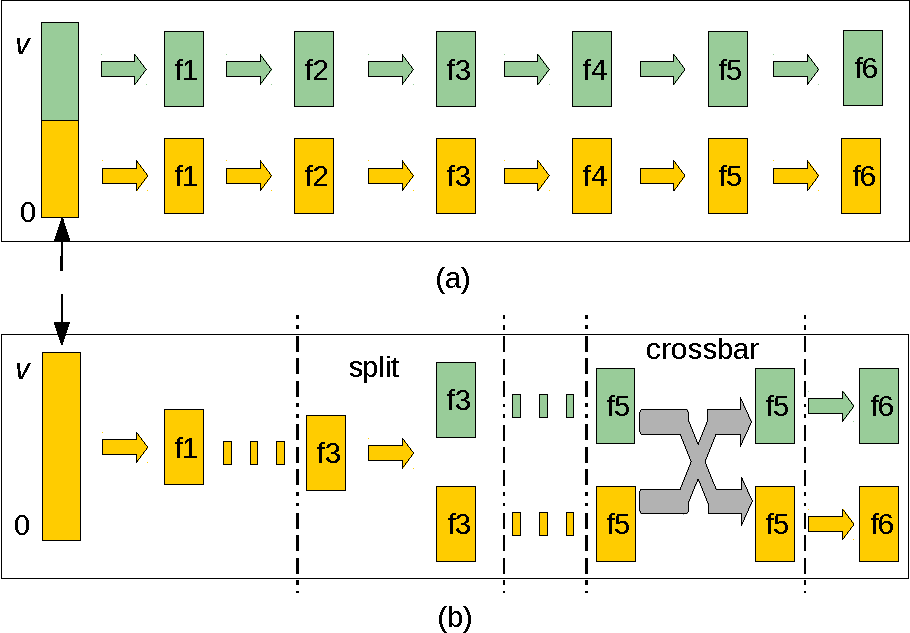
\includegraphics[width=0.85\linewidth]{pipeline-duplication}}
    \caption{pipeline duplication. (a) Straightforward pipeline duplication 
    (b) proposed pipeline duplication.}
\label{fig:duplicate-pipeline}
\end{figure}


\subsubsection{Data width optimization}
The memory bandwidth utilization is sensitive to the data width setup. 
According to our experience, sequential memory access 
with 512-bit data width consumes the optimal memory bandwidth. With this guideline, 
a lot of design parameters such as the cache line size and prefetch length are 
set to be 512-bit for higher memory bandwidth utilization. For the same reason, sequential 
memory access with smaller data width such as 32-bit integer is also 
padded and accessed with 512-bit global memory port.

\subsubsection{II optimization}
In the pipelined design, initialization interval (II) indicates the 
processing throughput. Larger II in a single pipeline stage 
may slow down the rest of the system. Thus we try to reduce II of all 
the pipelined sub functions. In particular, hash table, cache and prefetch 
buffer may affect the II. Inappropriate implementation may lead to 
large II and even compensate the benefits brought by these optimizations. 

\subsubsection{Deadlock removal}
Another challenge of the pipelined BFS accelerator design is the 
unexpected deadlock problem. 
When a pipeline stage issues a long burst request to the memory 
but gets stalled due to the insufficient read buffer, it has to 
wait for the downstream pipeline stages to consume the data in the buffer. 
However, the downstream pipeline stages may also be stalled due to 
the failure of acquiring the bus that is taken by the upstream pipeline stage.
It is difficult to debug and resolve this deadlock. To address this problem, we
add additional user buffer in the pipeline stages with long sequential 
memory access and split the long sequential memory access into smaller 
segments such that each segment can be accommodated by the buffer. 
Although this may cause slightly lower bandwidth utilization, it breaks the deadlock and 
ensures the correctness of the pipelined design.

\subsection{Parameter Tuning}
As presented in previous sub sections, there are quite some design 
parameters such as hash table size, cache design, prefetch 
length and II that need to be explored. However, exploring the design parameters 
based on the hardware implementation directly requires many lengthy 
hardware implementations (A typical BFS implementation may 
take 1 hour to 4 hours to complete.) which is extremely time-consuming.

In this work, we manually tune the design parameters. To obtain the 
optimized design parameters rapidly, we proposed a general HLS design 
parameter tuning flow for the HLS based design. The design flow is 
presented in Figure \ref{fig:parameter-tuning}. It includes three 
iterative loops tuning different types of the design parameters.

The first loop replies on the fast software emulation which is 
immediately available using HLS.
With the software emulation, we can extract a set of statistical 
metrics such as cache hit rate, prefetch hit rate that are 
mostly independent with the hardware implementation. These metrics can be used to 
guide the cache and prefetch buffer design. Although they 
are not sufficient to decide the exact accelerator performance, they 
can help prune the design options that are far from optimal and thus reduce 
the design parameter tuning time. The second tuning loop is based on the hardware 
pre-synthesis which is also fast and can be done in a few minutes. 
With the pre-synthesis report, we can optimize the II by 
improving the HLS design. When the potential design 
configurations gets smaller, we can get into the last loop and start the time consuming 
hardware implementation evaluating the configurations with the real 
performance or resource metrics. Finally, we would like to emphasize the verification process, 
it needs to be enabled all the time, as optimization may also cause mistakes of the resulting design.

\begin{figure}
\center{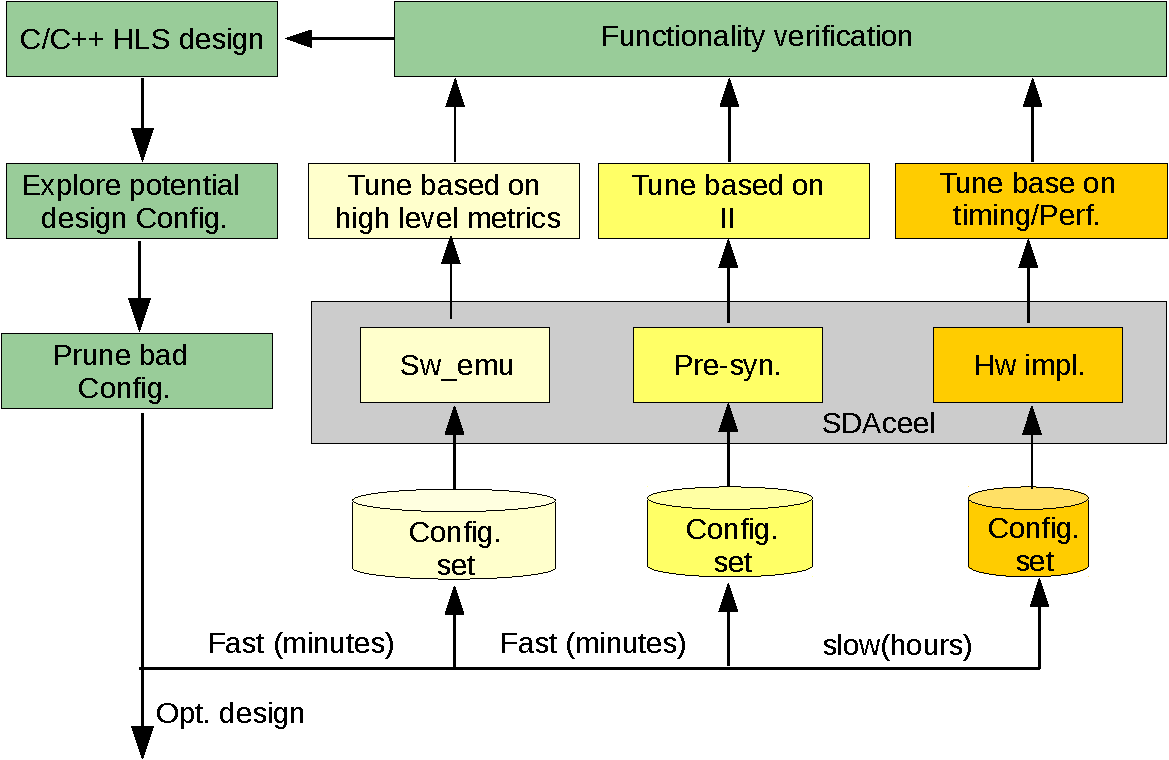
\includegraphics[width=0.95\linewidth]{parameter-tuning}}
    \caption{Design parameter tuning flow based on SDAccel.}
\label{fig:parameter-tuning}
\end{figure}


\section{Experiments} \label{sec:experiment}
In this section, we will measure the overall performance of the optimized 
HLS based BFS accelerator on Alpha Data ADM-PCIE-7v3 and 
compare it to a baseline HLS design using five skewed graphs which includes 
three real-world graphs and two graphs generated using R-MAT model \cite{chakrabarti2004rmat}.
In addition, we will also analyze and discuss the effect of the different HLS based 
BFS optimization techniques.

\subsection{Experiment Setup}
We use five skewed graphs listed in Table \ref{tab:graph} as the benchmark of this work. 
The real-world graphs are from social network \cite{yang2012defining, 
leskovec2009community, takac2012data} while the R-MAT graphs are generated 
using the Graph 500 benchmark parameters ($A=0.59, B=0.19, C=0.19$). We refer 
to an R-MAT graph with scale $S$ ($2^{S}$ nodes) and edge factor $E$ ($E\times 2^{S}$). 
In order to avoid trivial search, we only choose vertices from the largest 
connected component as the BFS starting point.

\begin{table}
  \caption{Skewed Graphs}
  \label{tab:graph}
  \begin{tabular}{cccl}
    \toprule
      Name & \# of vertex & \# of edge & Type \\
    \midrule
      Youtube \cite{yang2012defining} & 1157828 & 2987624 & Undirectional \\
      Live Journal \cite{leskovec2009community} & 4847571 & 68993773 & Directional \\
      Pokec \cite{takac2012data} & 1632804 & 30622564 & Directional \\
      rmat-19-32 & 524288 & 16777216 & Directional \\
      rmat-21-32 & 2097152 & 67108864 & Directional \\
  \bottomrule
\end{tabular}
\end{table}


\subsection{Overall Performance Comparison}
Overall performance comparison is presented in Figure \ref{fig:overall-performance}. 
The baseline is a single stage pipeline design, GAP is the optimized 
multi-core CPU implementation. The best performance speedup to a baseline design 
on the FPGA is up to 55X, but we are still far from the optimized multicore 
CPU implementation which is around 50X slower. I may remove the CPU results later. 

The big performance gap mainly comes from the low bandwidth utilization.
Currently, the best design I have consumes only around 300MB/s bandwidth 
which is around 3 percent of the peak memory bandwidth (10.8GB/s). We do have 
quite some space for improving.

\begin{figure}
\center{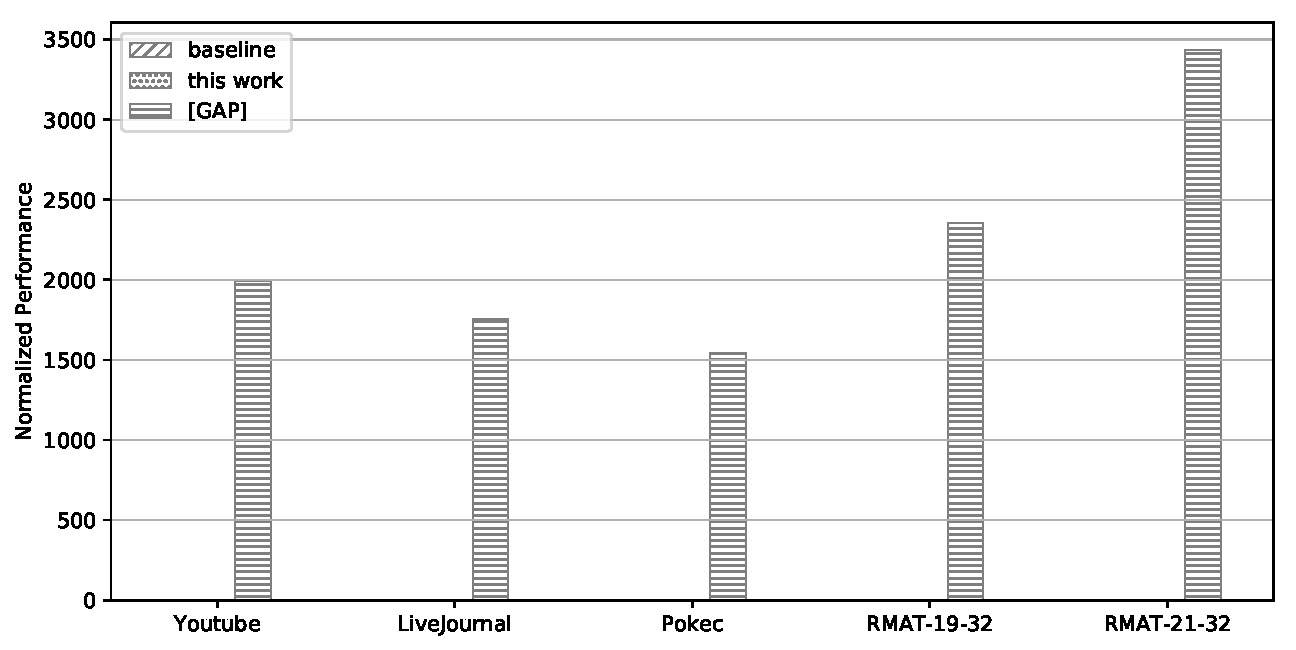
\includegraphics[width=0.95\linewidth]{overall-performance}}
    \caption{Performance Comparison. \textbf{4lane design is missing.} }
\label{fig:overall-performance}
\end{figure}

\begin{table}
  \caption{FPGA based BFS accelerator comparison}
  \label{tab:compare}
  \begin{tabular}{cccccc}
    \toprule
      Work & Platform & Graph & MTEPS & BW(GB/s) & MTEPS/BW \\
    \midrule
      \cite{betkaoui2012reconfigurable} & Convey HC-2 & RMAT & 1600 & 80  & 20 \\
      \cite{attia2014cygraph} & Convey HC-2 & RMAT    & 1900 & 80  & 24.4 \\
      \cite{umuroglu2015hybrid}      & Zedboard    & RMAT    & 172    & 3.2 & 53.7 \\
      \cite{zhang2017boosting} & Micro-AC510       & Random  & 166.2  & 60  & 2.8 \\
      \cite{dai2016fpgp}  & VC707 Kit & Twitter & 12  & 6.4 & 1.9 \\
      this work & ADM-PCIe-7v3 & RMAT & 30 & 10.8 & 2.9 \\
  \bottomrule
\end{tabular}
\end{table}


\subsection{Pipelining Analysis}
The pipelined BFS algorithm is beneficial to the HLS based implementation. 
However, an inappropriate pipelining strategy may have just marginal performance 
improvement while increasing the hardware overhead. In this work, we have implemented 
a number of pipelining strategies using HLS tools ranging from a single pipeline 
stage to 7 pipeline stages and then make comprehensive 
comparison among the implementations. The pipeline configurations 
are shown in Figure \ref{fig:pipeline-config} and the performance 
comparison is presented in Figure \ref{fig:pipeline-performance}.

\begin{figure}
\center{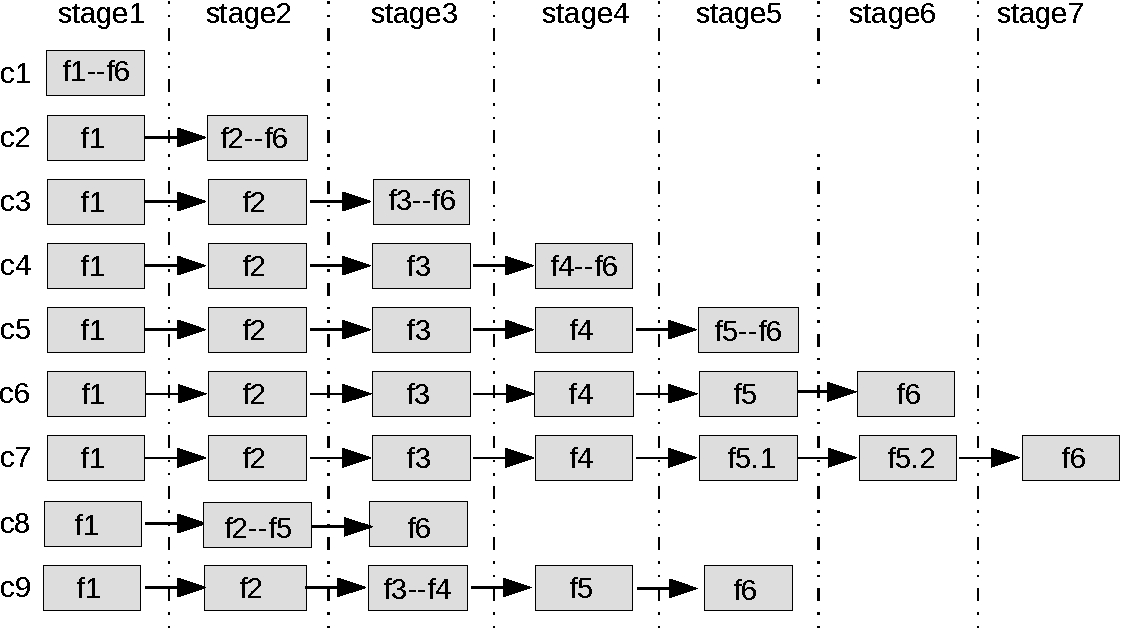
\includegraphics[width=0.95\linewidth]{pipeline-config}}
    \caption{Pipeline configurations with various combinations.}
\label{fig:pipeline-config}
\end{figure}

\begin{figure}
\center{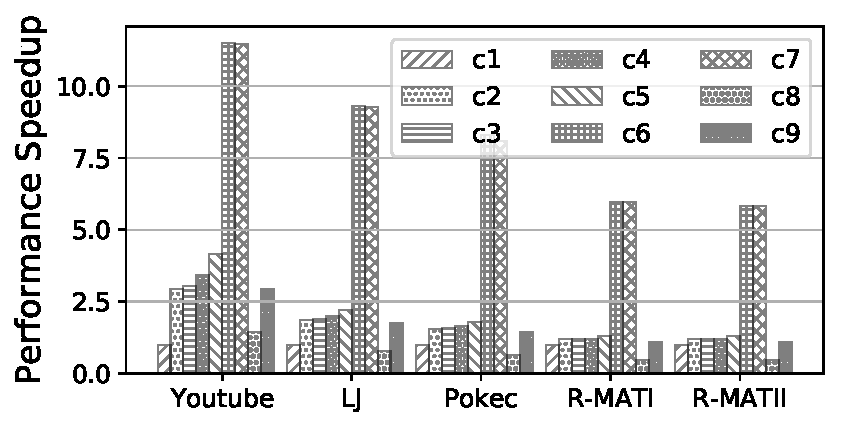
\includegraphics[width=0.95\linewidth]{pipeline-performance}}
    \caption{Performance speedup over a baseline design c1 which 
    is a best effort HLS implementation based on the native nested loop.}
\label{fig:pipeline-performance}
\end{figure}

\subsection{Hash Table Based Redundancy Removal}
There is a large proportion of redundant vertices in the frontier neighbors which 
are the major random memory access in BFS. We insert a hash table based filter to 
get rid of the redundant vertices such that the following time-consuming random memory access 
can be reduced. Figure \ref{fig:hash-redundancy} shows the overall redundancy 
removal percentage after the filter with different size of hash tables. It can be found that 
the redundancy removal is quite sensitive to the hash table size.
Nevertheless, the baseline implementation degrades when the hash table gets larger which 
even leads to the performance drop. The resulting performance is shown in Figure \ref{fig:hash-performance} 

\begin{figure}
\center{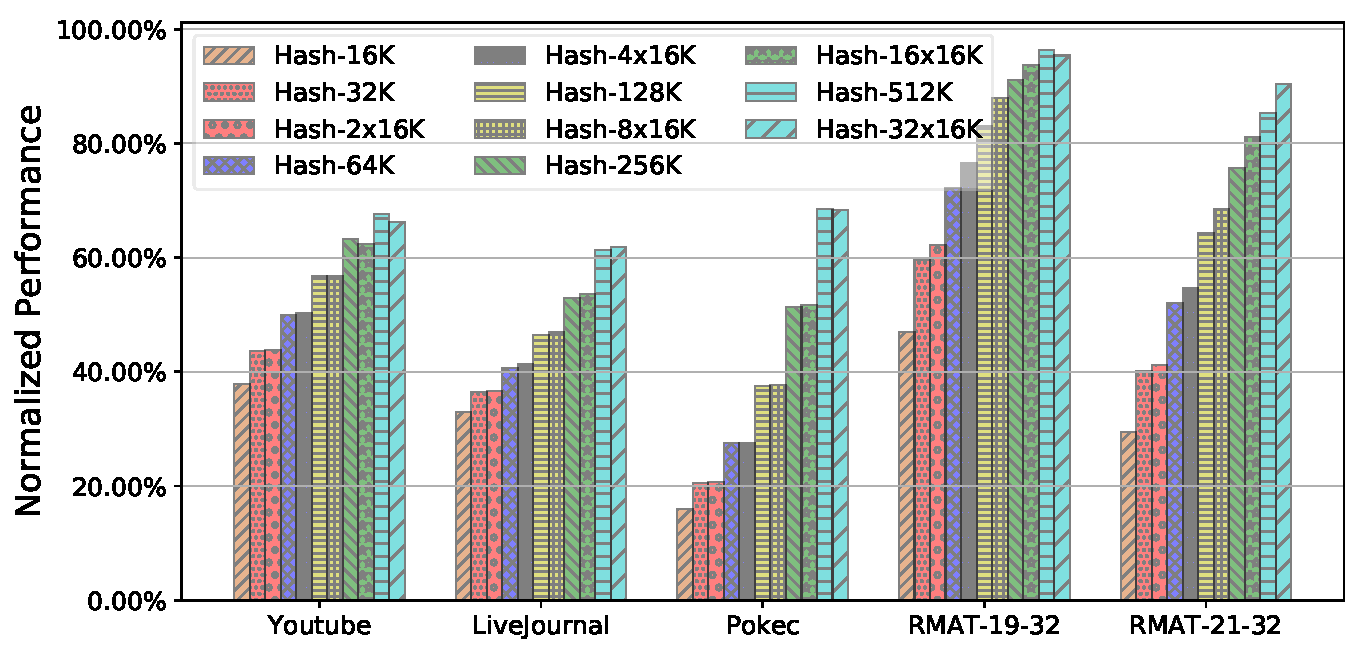
\includegraphics[width=0.95\linewidth]{hash-redundancy}}
    \caption{Redundancy neighbor vertices removal rate with the hash table based filters. 
    The redundancy removal rate is sensitive to the hash table size.}
\label{fig:hash-redundancy}
\end{figure}

\begin{figure}
\center{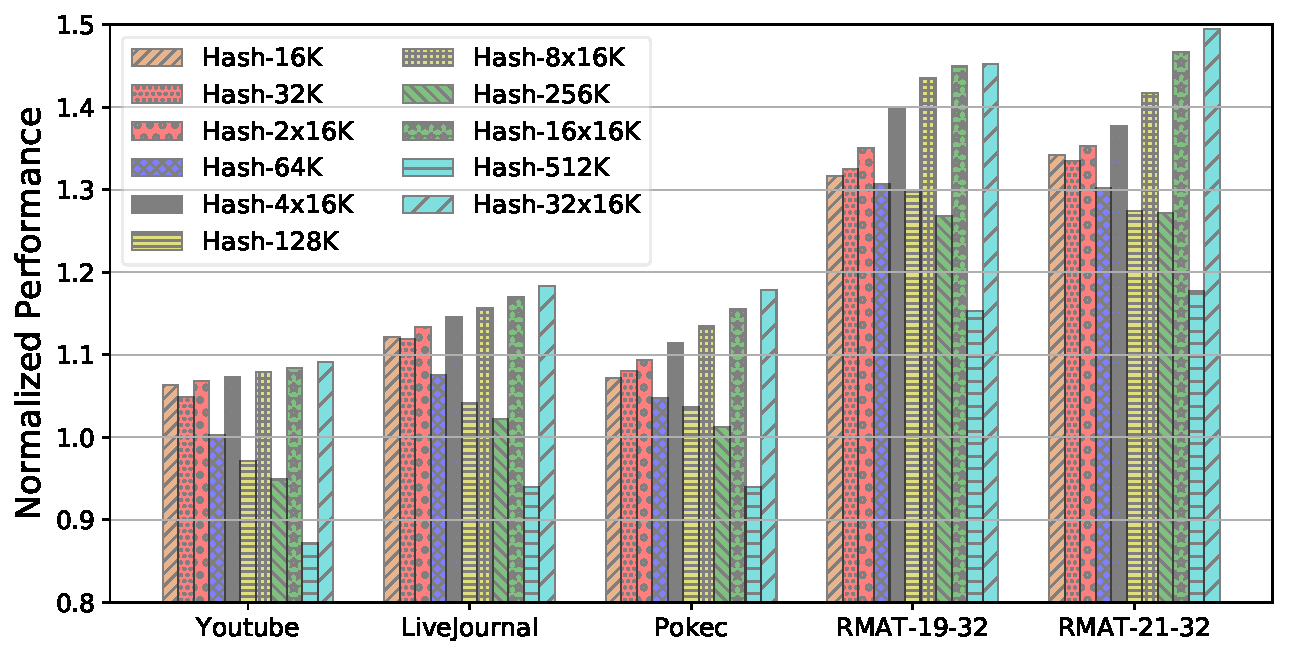
\includegraphics[width=0.95\linewidth]{hash-performance}}
    \caption{Resulting BFS performance with different hash table size}
\label{fig:hash-performance}
\end{figure}


\subsection{Memory access optimization}
Figure \ref{fig:cache-hit} shows the correlation between the 
cache and pre-fecth design parameter and the resulting cache 
hit rate. The influence varies slightly on different graph benchmark. 
With the hash and cache structure, the performance improves 2\~3X compared to 
the best pure pipleine design.

\begin{figure}
\center{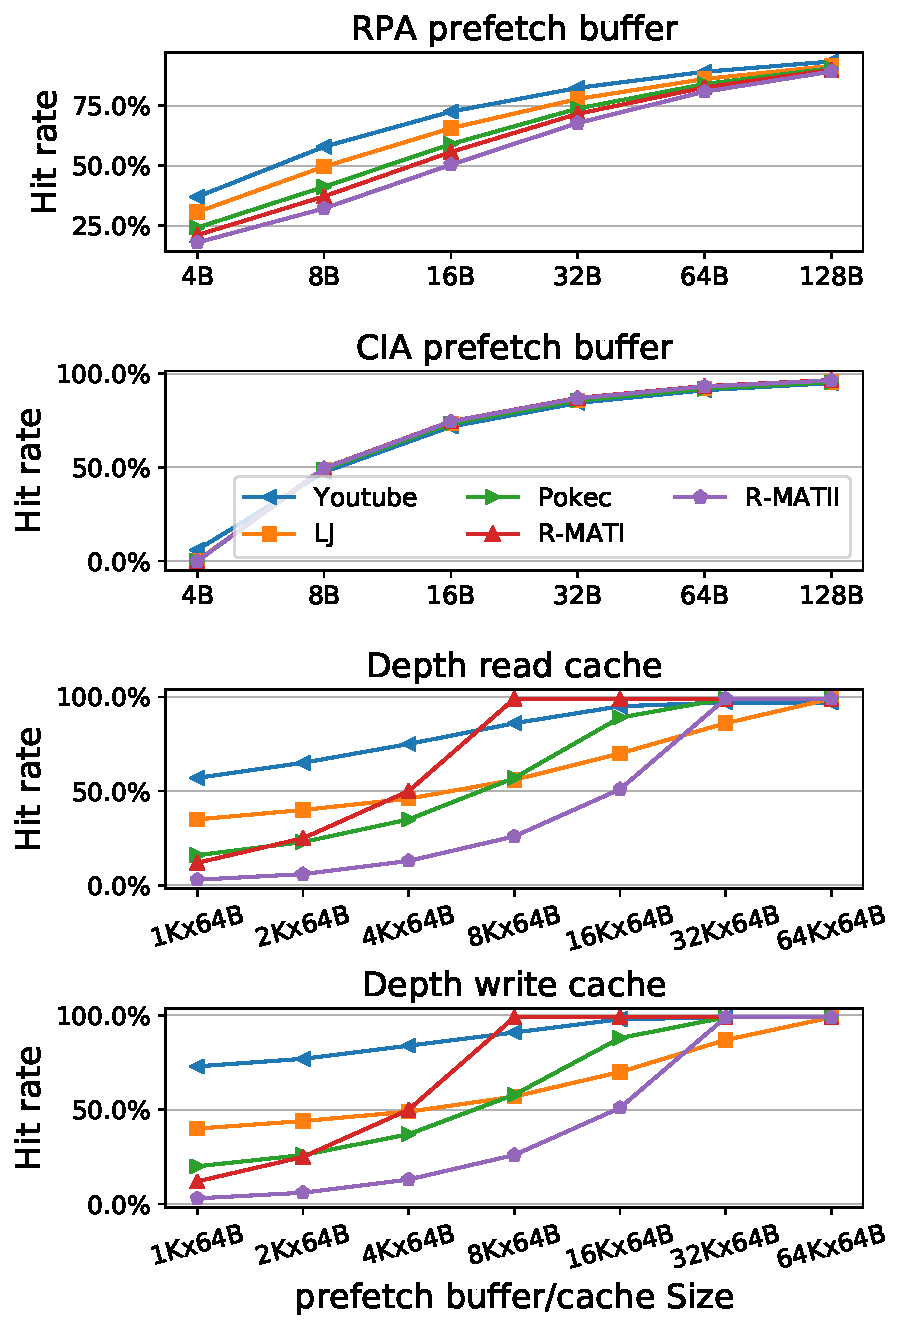
\includegraphics[width=0.95\linewidth]{cache-hit}}
    \caption{Cache and pre-fetch configurations have significant influence on the cache hit rate.
    The infleunce varies on different graph data set, but the trend is similar.}
\label{fig:cache-hit}
\end{figure}

Cache on the different bfs pipeline stages are benficial to the resulting performance.
Cache in S4, S5 and S6 improves the bfs performance dramatically as shown in 
Figure \ref{fig:cache-performance}.
\begin{figure}
\center{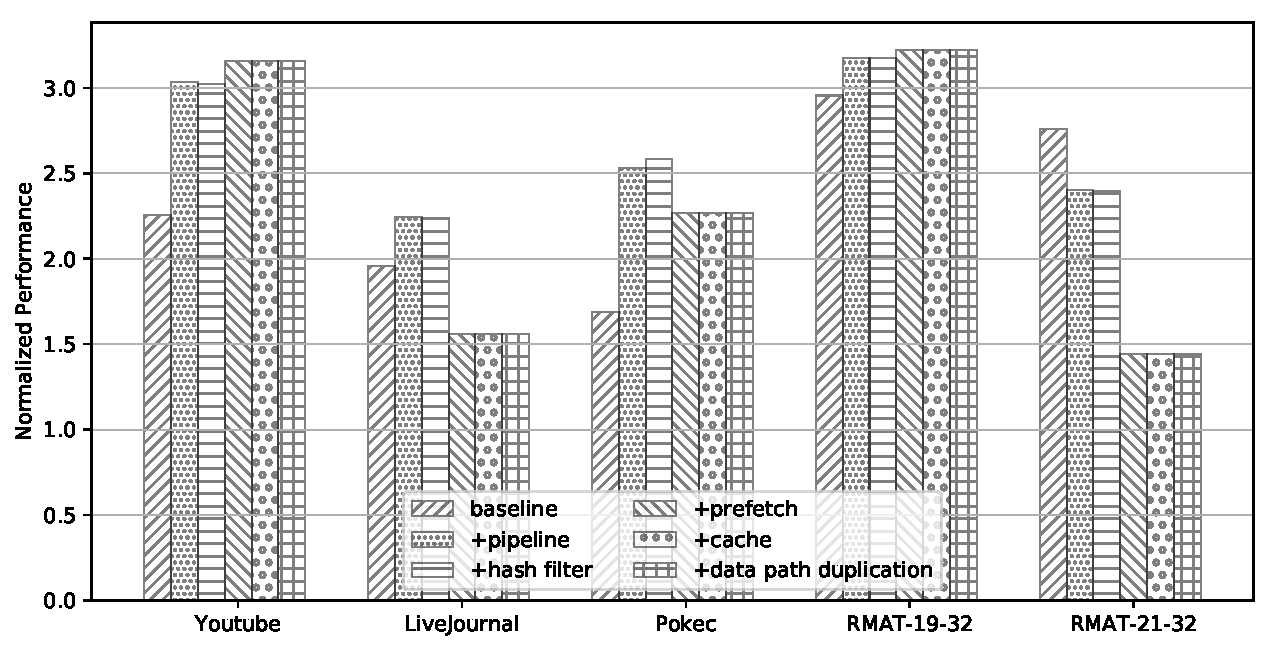
\includegraphics[width=0.95\linewidth]{cache-performance}}
    \caption{Cache in S4, S5 and S6 significantly imrpoves the bfs accelerator performance. 
    S2 is not on bottleneck and has little influence on the overall performance.}
\label{fig:cache-performance}
\end{figure}


\section{Conclusions} \label{sec:conclusion}
xxxxx

%\appendix
%\section{Acknowledgement}

%\begin{acks}
%  The authors would like to thank Sam Ho for providing the suggestions on
%  HLS design debugging and optimization as well as the SDAccel usage. 

%\end{acks}
